%% ------------------------------------------------------
%%	Document Latex créé par Paul Planchon (pdubs)
%%		le 24/04/2017 à Bordeaux
%%	      mis à jour de façon régulière
%%          Créditer l'auteur serait bienvenus
%% ------------------------------------------------------

\documentclass[11pt, a4paper]{article}

%% Tous les packages pour écrire en français %%%%%%%%%%%%
\usepackage[T1]{fontenc}
\usepackage[utf8]{inputenc}
\usepackage{lmodern}

%% Autres packages %%%%%%%%%%%%%%%%%%%%%%%%%%%%%%%%%%%%%
\usepackage[top = 50mm, headheight=62pt]{geometry}
\usepackage{titleps}
\usepackage{tabularx, booktabs, multirow}
\usepackage{graphicx, adjustbox, microtype}
\usepackage{lipsum}

%% Pour display du code %%%%%%%%%%%%%%%%%%%%%%%%%%%%%%%%
\usepackage{amsmath}
\usepackage{algorithm}
\usepackage[noend]{algpseudocode}
\makeatletter
\def\BState{\State\hskip-\ALG@thistlm}
\makeatother

%% Les deux colonnes %%%%%%%%%%%%%%%%%%%%%%%%%%%%%%%%%%%
\usepackage{multicol}
\usepackage{color}
\usepackage{comment}
\setlength{\columnseprule}{1pt}
\setlength{\columnsep}{0.5cm}
\def\columnseprulecolor{\color{black}}

%% Table des matières %%%%%%%%%%%%%%%%%%%%%%%%%%%%%%%%%%
\makeatletter
\renewcommand{\thesection}{\Roman{section}.}
\renewcommand{\thesubsection}{\Roman{section}.\arabic{subsection}.}
\renewcommand{\thesubsubsection}{\Roman{section}.\arabic{subsection}}
\makeatother

\makeatletter
\renewcommand{\section}{\@startsection{section}{1}{\z@}%
	{-3.5ex \@plus -1ex \@minus -.2ex}%
	{2.3ex \@plus .2ex}%
	{\reset@font\Large\bfseries	}}
\renewcommand{\subsection}{\@startsection{subsection}{1}{\z@}%
	{-3.5ex \@plus -1ex \@minus -.2ex}%
	{2.3ex \@plus .2ex}%
	{\reset@font\large\bfseries}}
\makeatother

\usepackage{hyperref}
\hypersetup{
    colorlinks,
    citecolor=black,
    filecolor=black,
    linkcolor=black,
    urlcolor=black
}

%% Titre %%%%%%%%%%%%%%%%%%%%%%%%%%%%%%%%%%%%%%%%%%%%%%%
\usepackage{fancyhdr}
\usepackage{lastpage}
\newpagestyle{style}{%
\sethead{}{%
\begin{tabularx}{\linewidth}[b]{@{}l>{\raggedleft\arraybackslash}X@{}}
\smash{\raisebox{-0.7\height}{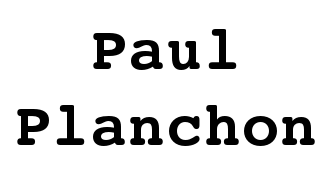
\includegraphics[scale=0.5]{logo.png}}}& \today \\
\cmidrule[2pt]{2-2}
& \huge \bfseries VID01 - Les fractales \\
& Thème: Mathématiques \& Java\\
\addlinespace
\midrule[0.4pt]
\end{tabularx}%
}{}
\setfoot{}{\thepage}{}
}%

%% Début du document %%%%%%%%%%%%%%%%%%%%%%%%%%%%%%%%%%
\usepackage[french]{babel}
\pagestyle{style}
\begin{document}
\tableofcontents

\section{Les mathématiques}
	\subsection{La fractale de Mandelbrot}
	\subsection{Les ensembles de Julia}

\section{Java}
	\subsection{L'utilisation de l'object}
	\subsection{Pseudo-code de l'algorithme}
	\subsection{Résultats}


	\section{Java}
		\subsection{L'utilisation de l'object}
		\subsection{Pseudo-code de l'algorithme}
		\subsection{Résultats}

\begin{multicols}{2}
Hello, here is some text without a meaning.  This text should show what
a printed text will look like at this place.
If you read this text, you will get no information.  Really?  Is there
no information?  Is there...
\end{multicols}

\begin{algorithm}
\caption{My algorithm}\label{euclid}
\begin{algorithmic}[1]
\Procedure{MyProcedure}{}
\State $\textit{stringlen} \gets \text{length of }\textit{string}$
\State $i \gets \textit{patlen}$
\BState \emph{top}:
\If {$i > \textit{stringlen}$} \Return false
\EndIf
\State $j \gets \textit{patlen}$
\BState \emph{loop}:
\If {$\textit{string}(i) = \textit{path}(j)$}
\State $j \gets j-1$.
\State $i \gets i-1$.
\State \textbf{goto} \emph{loop}.
\State \textbf{close};
\EndIf
\State $i \gets i+\max(\textit{delta}_1(\textit{string}(i)),\textit{delta}_2(j))$.
\State \textbf{goto} \emph{top}.
\EndProcedure
\end{algorithmic}
\end{algorithm}

\lipsum[1]

\end{document}
